\documentclass{article}
\usepackage{pdfpages}
\usepackage{verbatim}
\begin{document}
	\begin{center}
		\begin{LARGE}
			\textbf{HW3}\\
		\end{LARGE}
		Yao, Yi\\
		sakfljklasdj
	\end{center}
	\begin{enumerate}
		\item 
		Introduction:\\
		This software simulates the operation of a north-south-one-lane bridge, whose capacity , as well as the north and south input buffers (queues) are in theory $+\infty$. When one side ends traversing the bridge, the other side starts traversing if cars are present in queue, otherwise, the same side starts traversing, if cars are present in queue. The model is implemented using Event Scheduling based Discrete Event Simulation.
		\item 
		
	\end{enumerate}
	\verbatiminput{test.txt}
	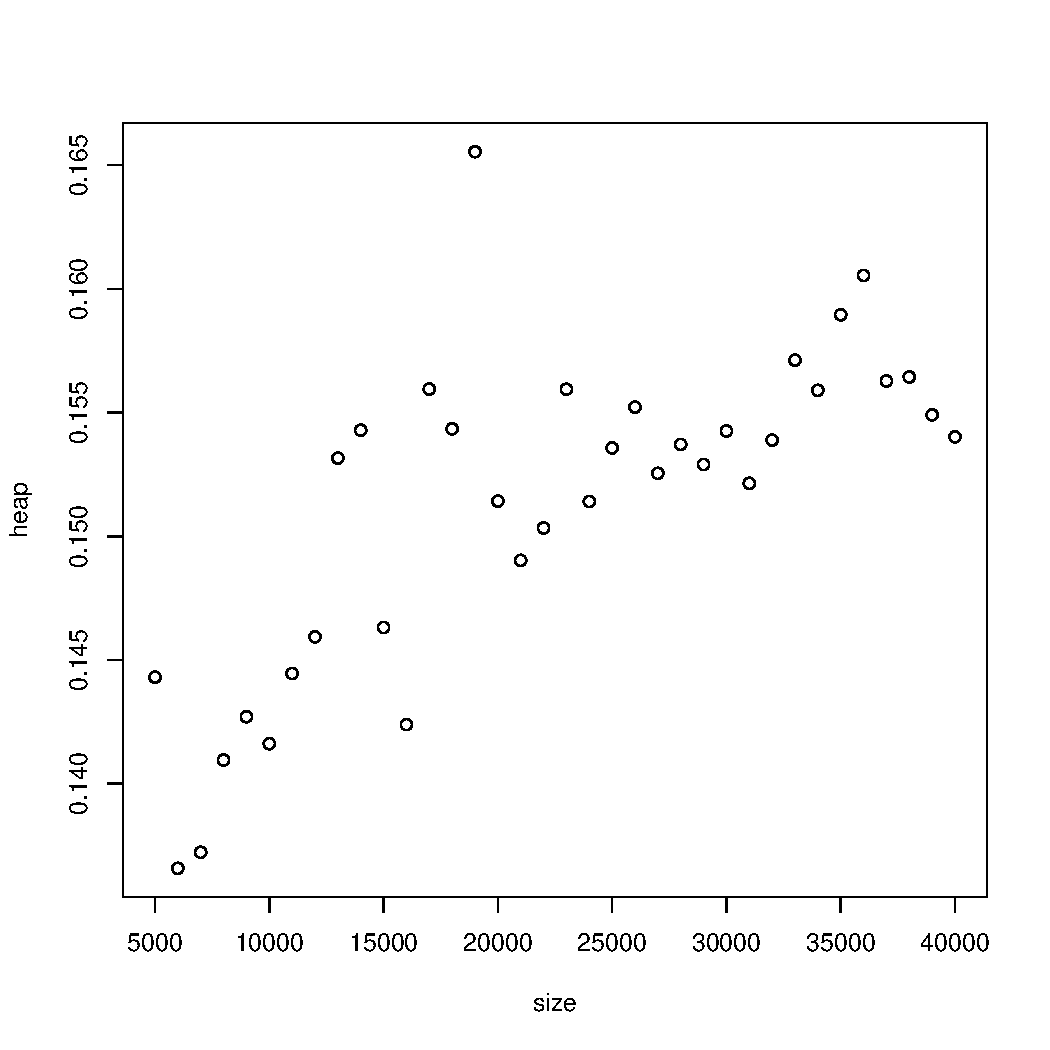
\includepdf[pages=-]{Rplots.pdf}
\end{document}